\mychapter{Redes Neurais Artificiais}
\label{cap:rnas}

Ao longo das últimas décadas, as pesquisas na área de Redes Neurais Artificiais
(RNAs) evoluiram de maneira significativa, principalmente após a década de 80,
com o avanço da tecnologia e o fracasso da escola simbolista na solução de
determinados tipos de problemas \cite{braga:2007}.

No setor industrial a história não foi muito diferente. As RNAs vem sendo
utilizadas em diversos trabalhos, seja de maneira isolada ou em sistemas
híbridos, os quais combinam outras características de sistemas inteligentes,
tais como técnicas {\it Fuzzy} ou Algoritmos Genéticos.

Neste capítulo serão mostrados, de maneira resumida, os conceitos que envolvem
as RNAs, destacando algumas de suas propriedades e atributos. Por fim a atenção
será voltada para o modelo que será utilizado para a identificação da dinâmica
do processo e das falhas.

% ------------------------------------------------------------------------------
\section{Conceitos fundamentais}
Segundo \citeasnoun{haykin:2000}, as RNAs são estruturas paralelas, maciçamente
distribuídas, constituídas por unidades simples de processamento conhecida como
neurônios. Essas estruturas se assemelham ao cérebro humano devido a sua
capacidade de ``adquirir conhecimento'' a partir do ambiente em que se encontra.
Esse aprendizado ocorre através de um ajuste das forças de conexões, ou pesos
sinápticos, que existe entre os neurônios. São essas conexões que armazenam os
conhecimentos adquiridos pela rede.

Dentre as diversas aplicações das RNAs, podem ser citados exemplos para a
classificação de padrões, filtragem de sinais, análise de imagens, identificação
e controle de sistemas dinâmicos. De acordo com \citeasnoun{haykin:2000},
algumas das justificativas para a utilização dessas estruturas são: sua
característica intrínseca de não-linearidade, sua capacidade de generalização e
adaptabilidade, a tolerância à falhas e a facilidade para realizar o mapeamento
de relações entrada-saída.

Devido à grande complexidade existente em muitos problemas físicos reais,
desenvolver um modelo matemático que represente adequadamente a dinâmica do
processo é uma tarefa praticamente impossível. Para \citeasnoun{reboucas:2009},
as RNAs, através de seu processo de aprendizagem e de sua capacidade de
aproximação universal, conseguem representar a função correspondente à dinâmica
do sistema com relativa simplicidade.

\begin{comment}
Pode-se dizer que essa capacidade de aproximação assemelha a funcionalidade de
um sistema de inferência, que nada mais é do que um modelo capaz de reproduzir
as relações dinâmicas existentes entre as variáveis primárias e as variáveis
secundárias de um processo.
\end{comment}

Apesar de se conhecer as equações que regem a dinâmica do processo escolhido
como estudo de caso deste trabalho, conforme será mostrado no Capítulo
\ref{cap:sistema}, justifica-se desde já a utilização de RNAs para identificação
do modelo em virtude da necessidade de simulação das falhas. Maiores detalhes
serão esclarecidos ao longo do texto do referido capítulo.

% ------------------------------------------------------------------------------
\section{Arquitetura das redes}
Dentre as diversas arquiteturas de redes neurais existentes, tais como as redes
de funções de base radial, as redes de Kohonen, máquinas de vetor de suporte,
dentre outras, a arquitetura escolhida para este trabalho foi a das redes
Perceptron de Múltiplas Camadas (PMC), treinadas com o algoritmo
Levenberg-Marquardt (LMA) disponível no {\it software} matemático Matlab\reg. A
Fig. \ref{fig:pmc} representa um modelo esquemático de uma rede PMC.

\begin{figure}[htb]
\centering
    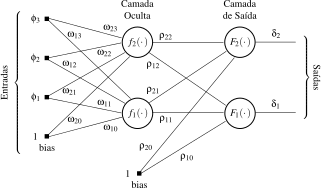
\includegraphics[width=0.65\textwidth]{imgs/rnas/eps/pmc}
    \caption{Diagrama esquemático de uma rede PMC.}
    \label{fig:pmc}
\end{figure}

\Glossary{PMC}{Perceptron de Múltiplas Camadas}
\Glossary{LMA}{Levenberg-Marquardt}

A opção pela estrutura de PMC se dá devido a sua simplicidade e capacidade de
aplicação em diversas áreas. Já a opção pelo treinamento com o algoritmo LMA
pode ser justificada por se tratar de um método Quase-Newton que acelera o
processo de convergência da rede, uma vez que leva em consideração termos de
ordens mais elevadas que o algoritmo {\it backpropagation}. 

Ademais, pode-se comentar que, apesar de ser possível realizar o treinamento das
redes através de uma linguagem de programação convencional, implementar tais
soluções, tão difundidas em {\it softwares} mundialmente reconhecidos como o
Matlab\reg\ e amplamente aceitas no meio acadêmico, está fora do escopo deste
trabalho.

Segundo \citeasnoun{norgaard:2000}, uma rede PMC básica possui seus neurônios
dispostos em camadas, recebendo como entrada as saídas dos neurônios da camada
imediatamente anterior ou, no caso da primeira camada, as entradas da rede. Por
possuir essa configuração essas redes são conhecidas como redes {\it
feedforward}.

Como mostrado na Fig. \ref{fig:pmc}, a segunda camada é conhecida como camada
de saída, pois produz as saídas da rede neral. A primeira camada é conhecida
como camada oculta ou intermediária por estar ``escondida'' entre as entradas da
rede ($\phi_1$, $\phi_2$ e $\phi_3$) e a camada de saída. Em
\citeasnoun{cybenko:1989} foi demonstrado que qualquer função contínua pode ser
aproximada por uma rede neural PMC que possua uma camada oculta com funções de
ativação sigmoidal ou tangente hiperbólica.

A Eq. \ref{eq:func_rede_pmc} expressa matematicamente o funcionamento de uma
rede neural PMC de duas camadas, como na Fig. \ref{fig:pmc}, em que $\delta_i$
representa a $i$-ésima saída da rede.

\begin{equation}\label{eq:func_rede_pmc}
\delta_i(t) = g_i[\phi,\theta] =
              F_i\colchete{\sum_{j=1}^{n_h}\rho_{i,j}f_j
              \parent{\sum_{l=1}^{n_\phi}\omega_{j,l}\phi_l+\omega_{j,0}}+
              \rho_{i,0}}
\end{equation}
\Glossary{$\delta_i$}{$i$-ésima saída da rede neural}
\Glossary{$\phi$}{Vetor de entradas da rede neural}
\Glossary{$\phi_l$}{$l$-ésima entrada da rede neural}
\Glossary{$\theta$}{Vetor de parâmetros ajustáveis da rede neural}
\Glossary{$F$, $f$}{Funções de ativação dos neurônios da rede neural}
\Glossary{$\rho$}{{\it biases}}
\Glossary{$\rho_{i,j}$}{{\it biases} que partem da camada $j$ e chegam na camada
                        $i$}
\Glossary{$\omega_{j,l}$}{Peso sináptico que parte do neurônio $l$ e chega no
                          neurônio $j$}
\Glossary{$n_h$}{Número de neurônios da camada oculta}
\Glossary{$n_\phi$}{Número de entradas da rede}

O vetor de parâmetros $\theta$ contém os pesos sinápticos e {\it biases}
($\omega_{j,l}$, $\rho_{i,j}$). O número de neurônios da camada oculta e o
número de entradas da rede são, respectivamente, $n_h$ e $n_\phi$, enquanto que
$F_i$ e $f_j$ são as funções de ativação dos neurônios das camadas de saída e
oculta, respectivamente. As funções de ativação mais comumente utilizadas são
mostradas nas equações \ref{eq:lin}, \ref{eq:sig} e \ref{eq:tan}.

\begin{equation}
\label{eq:lin}
f_l(x)=x \\
\end{equation} 

\Glossary{$f_l$}{Função de ativação linear}

\begin{equation}
\label{eq:sig}
f_s(x) = \frac{1}{1+e^{-x}}\\
\end{equation} 

\Glossary{$f_s$}{Função de ativação sigmoidal}

\begin{equation}
\label{eq:tan}
f_t(x) = \text{tanh}(x) = \frac{1-e^{-x}}{1+e^{-x}}\\
\end{equation}

\Glossary{$f_t$}{Função de ativação tangente hiperbólica}

% ------------------------------------------------------------------------------
\section{Identificação através de modelo neural}
\begin{comment}
Segundo \citeasnoun{reboucas:2009}, a realização de inferência utilizando RNAs
pode ser vista como um problema de identificação, uma vez que a rede neural
treinada deve ser capaz de representar, satisfatoriamente, a dinâmica existente
entre as variáveis secundárias e primárias do processo.
\end{comment}

Segundo \citeasnoun{reboucas:2009}, as estruturas de modelo baseadas em redes
neurais, apropriadas para a identificação de sistemas não-lineares, são
generalizações de modelos lineares.  Para \citeasnoun{lucena:2005}, essas
estruturas são caracterizadas por seu vetor de regressão, que nada mais é do que
um vetor que contém as variáveis utilizadas para estimar a saída do sistema.
Dependendo da escolha do vetor de regressão, diferentes estruturas de modelo
neural podem surgir. Estruturas FIR ({\it Finite Impulse Response}), ARX ({\it
AutoRegressive eXternal input}), ARMAX ({\it AutoRegressive Moving Average
eXternal input}), OE ({\it Output Error}) e SSIF ({\it State Space Innovations
Form}) são algumas das estruturas lineares mais conhecidas. Se o vetor de
regressão for selecionado para modelos ARX, a estrutura do modelo neural será
chamada NNARX ({\it Neural Network ARX}). Do mesmo modo, existirão também
modelos NNFIR, NNARMAX, NNOE e NNSSIF.

\Glossary{FIR}{{\it Finite Impulse Response}}
\Glossary{ARX}{{\it AutoRegressive eXogenous}}
\Glossary{ARMAX}{{\it AutoRegressive Moving Average eXogenous}}
\Glossary{OE}{{\it Output Error}}
\Glossary{SSIF}{{\it State Space Innovations Form}}
\Glossary{NNARX}{{\it Neural Network AutoRegressive eXogenous inputs}}
\Glossary{NNARMAX}{{\it Neural Network AutoRegressive Moving Average eXogenous
                        inputs}}
\Glossary{NNOE}{{\it Neural Network Output Error}}
\Glossary{NNSSIF}{{\it Neural Network State Space Innovations Form}}

Neste trabalho foi utilizado um modelo de rede baseado no NNARX descrito em
\citeasnoun{norgaard:2000}. A Fig. \ref{fig:nnarx} representa um esquema
simplificado do modelo adotado. A presença de regressores no modelo, relaciona a
saída da rede com seus valores passados de entrada e saída. A utilização desses
regressores é de fundamental importância para a identificação de sistemas.

\begin{figure}[htb]
\centering
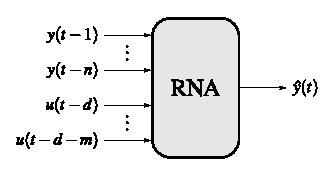
\includegraphics[width=0.45\textwidth]{imgs/rnas/eps/nnarx}
\caption{Esquema de uma rede neural com estrutura NNARX.}
\label{fig:nnarx}
\end{figure}

\Glossary{$y$}{Saída da planta}
\Glossary{$u$}{Entrada da planta}
\Glossary{$d$}{Atraso de transporte}

A expressão matemática que descreve o modelo não-linear pode ser descrita
conforme Eq. \ref{eq:modelo_nnarx}.

\begin{equation}
\label{eq:modelo_nnarx}
\hat{y}(t) = g\parent{y(t-1), \ldots, y(t-n), u(t-d), \ldots, u(t-d-m)}
\end{equation}

\Glossary{$\widehat{y}(t)$}{Saída estimada pela rede neural}
\Glossary{$n$}{Ordem de saída}
\Glossary{$m$}{Ordem de entrada}

Nessa equação $\hat{y}$ representa a saída estimada, $d$ o atraso de transporte,
$n$ a ordem da saída, $m$ a ordem de entrada da planta, $g( \cdotp )$ uma função
não linear mapeada pela rede neural, $y$ a saída da planta e $u$ a entrada da
planta.

A estimativa gerada pela estrutura NNARX é sempre estável, uma vez que
representa relações puramente algébricas entre a estimativa e as medições
passadas de entradas e saídas do processos, não existindo a realimentação da
saída estimada.

% ------------------------------------------------------------------------------
\subsection{Determinação da ordem do modelo}
\label{sec:det_ordem}
Em sistemas de identificação {\it blackbox}\footnote{Também conhecida como
identificação em caixa-preta, a identificação {\it blackbox} pressupõe que não
se dispõe de nenhuma informação sobre a estrutura interna ou sobre o
funcionamento do sistema. Nesse tipo de abordagem, faz-se uso de uma análise da
relação dos valores de saída obtidos a partir dos estímulos fornecidos nas
entradas do sistema.}, como o utilizado neste trabalho, é de fundamental
importância que a ordem do modelo seja determinada adequadamente.  Uma escolha
inadequada poderá fazer com que a dinâmica do processo não seja assimilada pela
rede neural, fazendo com que as estimativas geradas possuam erro médio
consideravelmente alto. Segundo \citeasnoun{arruda:2003}, existe uma ordem de
modelo ótima que permite obter o menor erro entre o modelo estimado e o sistema
real.

A ordem de entrada ($m$) e de saída ($n$) de um sistema desse tipo pode ser
obtida a partir da realização de testes ou simulações com o processo. Por
facilidade de representação, considerar-se-á a ordem de entrada igual a ordem de
saída ($m = n$). No capítulo \ref{cap:resultados} poderão ser vistos alguns
resultados dos testes que foram realizados para a determinação da ordem das
redes de identificação e de detecção e diagnóstico de falhas.

% ------------------------------------------------------------------------------
\subsection{Seleção do modelo}
Existem diversas estruturas de modelagem, cada uma com suas vantagens e
desvantagens. Segundo \citeasnoun{norgaard:2000}, o problema da seleção das
estruturas pode ser dividido em duas partes. A primeira delas é a parte da
seleção da ``família'' de estruturas de modelagem. Dependendo do sistema, as
estruturas podem ser: modelos lineares, redes PMC, redes de função de base
radial, {\it wavelets} etc. Já a segunda, é a parte da seleção do subconjunto da
família escolhida.

A escolha por uma estrutura do tipo NNARX se deu pelas diversas vantagens em se
utilizar RNAs para estimar valores e por se tratar de um modelo que não faz uso
de realimentação da saída estimada, o que permite dizer que este é estável no
sentido BIBO\footnote{Um sistema é dito BIBO estável quando, para qualquer
entrada limitada, obtém-se uma saída também limitada.} ({\it Bounded Input,
Bounded Output}). Para \citeasnoun{norgaard:2000}, devido a estas
características, o modelo NNARX é um dos mais utilizados quando o sistema a ser
modelado é determinístico ou o nível de ruído não é significativo.

\Glossary{BIBO}{\it Bounded Input, Bounded Output}

De maneira resumida, após a seleção da estrutura, segue-se uma sequência de
etapas até que o modelo possa representar adequadamente o sistema, de acordo com
algum critério específico, como por exemplo, o erro médio quadrático (EMQ) de
estimativa, que é calculado a partir da Eq. \ref{eq:emq} e utilizado no
algoritmo de treinamento da RNA para determinar o ponto de parada (fim do
treinamento).

\Glossary{EMQ}{Erro Médio Quadrático}

\begin{equation}\label{eq:emq}
\text{EMQ} = \sqrt{\frac{1}{N}
             \sum_{i=1}^{N}\pfrac{y_i - \widehat{y_i}}{y_i}^2}
\end{equation}

Nessa equação, $N$ representa o número de amostras de validação, $y_i$ o valor
real e $\widehat{y_i}$ o valor estimado.

\Glossary{$N$}{Número de amostras de validação}
\Glossary{$y_i$}{$i$-ésimo valor real de saída da planta}
\Glossary{$\widehat{y_i}$}{$i$-ésimo valor estimado pelo sistema}

Tendo conhecido as características das redes neurais que serão utilizadas no
desenvolvimento deste trabalho, o capítulo seguinte trará os principais
conceitos e terminologias relacionadas ao tema de detecção e diagnóstico de
falhas.
